\documentclass[10pt,letterpaper]{article}
\usepackage[top=1in,bottom=1in,left=1in,right=1in]{geometry}
\usepackage{datetime}
\usepackage{natbib}      % http://merkel.zoneo.net/Latex/natbib.php
\usepackage{palatino}
\usepackage{verbatim}
\usepackage[normalem]{ulem}
\bibpunct{(}{)}{;}{a}{,}{,}

\usepackage{array}

\usepackage{chngpage}
\usepackage{stmaryrd}
\usepackage{amssymb}
\usepackage{amsmath}
\usepackage{graphicx}
\usepackage{lscape}
\usepackage{subfigure}
\usepackage[usenames,dvipsnames]{color}
\definecolor{myblue}{rgb}{0,0.1,0.6}
\definecolor{mygreen}{rgb}{0,0.3,0.1}
\definecolor{mygray}{rgb}{0.2, 0.2, 0.2}
\usepackage[colorlinks=true,linkcolor=myblue,citecolor=mygray,urlcolor=myblue]{hyperref}


\newcommand{\bocomment}[1]{\textcolor{Bittersweet}{BO says: #1}}

\newcommand{\ignore}[1]{}
\newcommand{\transpose}{^\mathsf{T}}
\newcommand{\inner}[1]{\langle #1 \rangle}
\newcommand{\smallsec}[1]{\noindent \textbf{#1\ }}
\newcommand{\cmd}[1] {{\color{mygray}\texttt{#1}}}
\newcommand{\solution}[1]{{\color{myblue} \emph{[Solution:}
#1

\emph{End solution]}}}
\newcommand{\solutionnote}[1]{{\color{myblue} \emph{[Note:}

#1

\emph{End note]}}}
\newcommand{\points}[1]{{\color{mygreen}\emph{[#1]\ \ }}}

\newcommand{\aone}{\diamondsuit}
\newcommand{\atwo}{\heartsuit}
\newcommand{\bone}{\triangle}
\newcommand{\btwo}{\Box}
\newcommand{\myand}{\ \land\ }
\newcommand{\myor}{\ \lor\ }
\newcommand{\mynot}{\lnot}

\title{
  \Large{\textbf{CS4501-003: Computer Vision, Spring 26 @ UVA}}\\
 \textbf{Homework 2}\\
  \vspace{0.5em}
  \large{Instructor: Zezhou Cheng} \\
  \large{TAs: Jin Yao, Boyang Wang, Xuweiyi Chen}
}

\settimeformat{ampmtime}
\date{}
\begin{document}
\maketitle
\vspace{-10mm}

\renewcommand\thesubsection{\thesection.\alph{subsection}}

\section{Short answers [10 points]}
Answer the following questions. Each question will be graded as \emph{right} (100\% points),
\emph{mostly right} (50\% point), and \emph{wrong} (0\% points).

\begin{enumerate}
  \item \points{3 points} Implement the following using image filtering / 2D convolution.\\
  (You may find \cmd{scipy.signal.convolve2d} useful for this.)
    \begin{itemize}
        \item Spatial gradient along X axis using a $3 \times 3$ filter
    	\item Spatial gradient along Y axis using a $3 \times 3$ filter (You could use either Prewitt or Sobel filter in our \hyperlink{https://www.dropbox.com/scl/fi/pe70jjp9a241xz86hc8c2/lec7.pdf?rlkey=z4lmzl57txlrodbwn5w5si3jm&e=1&st=9um9kpnx&dl=0}{lecture 7}  )
    	\item Average values at each pixel location over a $5 \times 5$ window
    \end{itemize}

    Show the values in the filter kernel as a $k \times k$ matrix and the
    output of each for the image below.

    \begin{figure}[h]
    	\centering
    	
\includegraphics[width=5cm]{fig/hw0405_cat.png}
    	\caption{ Image source: https://favim.com/image/6683763/}
    \end{figure}

    \item \points{2 points} Explain how increasing the size of an averaging filter affects image noise and detail. Why might a larger filter not always be better?
    
    
    \item \points{5 points} Show that filtering an image with a separable 2D filter kernel is equivalent to filtering it with two 1D filter kernels, with mathematical justification. 

\end{enumerate}

\section{Scale-space blob detection [45 points]}




\begin{figure}[h]
\centering
\begin{tabular}{cc}
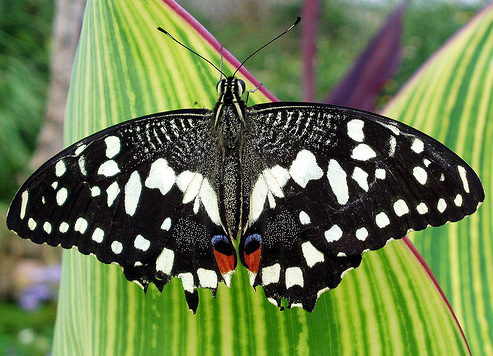
\includegraphics[width=0.4\linewidth]{./fig/butterfly.jpg} &
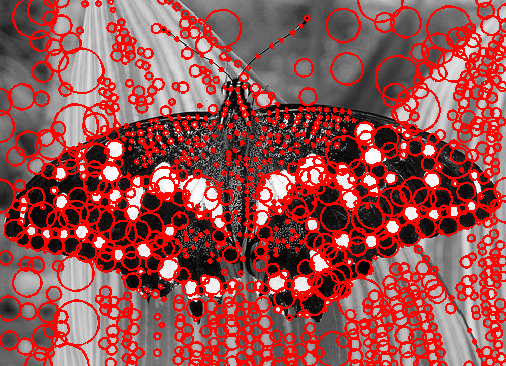
\includegraphics[width=0.4\linewidth]{./fig/butterfly.png} \\
\end{tabular}
\caption{\label{fig:blobs} Scale-space blobs detection}
\end{figure}




In this homework you will implement a simple panoramic image stitching algorithm. The first part is to detect blobs as keypoints. The algorithm is outlined as follows:


\begin{enumerate}
\item Build a Laplacian scale space, starting with some initial scale and going for n iterations:
\begin{enumerate}
\item Filter image with scale-normalized Laplacian at current scale.
\item Save the square of Laplacian response for current level of scale space.
\item Increase scale by a factor k.
\end{enumerate}
\item Perform non-maximum suppression in scale space.
\item Display resulting circles at their characteristic scales for points above a threshold.
\end{enumerate}


\paragraph{Test images.} There are four images in the folder \cmd{data/blobs} to test your code. Fig.~\ref{fig:blobs} provides the output of "butterfly" example as a reference to debug your code. Keep in mind that your output may look different depending on your threshold, range of scales, and other implementation details.


\paragraph{Running the code.} Start from the entry code \cmd{evalBlobsDetection}. It calls the dummy implementation of \cmd{detectBlobs} and draws the blob with \cmd{drawBlobs} as Fig.~\ref{fig:dummy}. You will need to install \cmd{scikit-image} and \cmd{OpenCV} by \cmd {conda install scikit-image} and \cmd{conda install -c menpo opencv}. You need to implement the function in \cmd{detectBlobs} which outputs a $n \times 4$ matrix with a blob in each row as (x, y, radius, score). 


\begin{figure}[h]
\centering
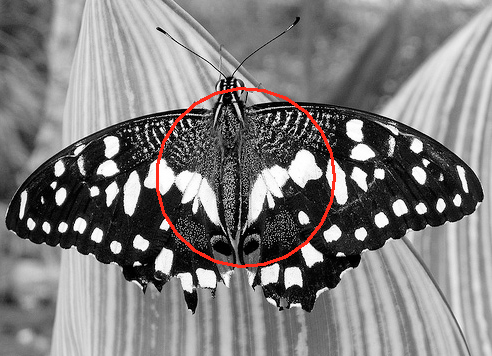
\includegraphics[width=0.3\linewidth]{./fig/butterfly-dummy.png} 
\label{fig:dummy}
\caption{\label{fig:dummy} Output of running the default implementation of evalBlobsDetection}
\end{figure}


The following are the hints to implement the function:


\begin{itemize}
\item Don't forget to convert images to gray-scale and double. 
%(\cmd{rgb2gray} command) (\cmd{im2double}).
\item For creating the Laplacian filter, you may use the function \cmd{scipy.ndimage.generic\_laplace} or \cmd{cv2.Laplacian}. Pay careful attention to setting the right filter size.
%\cmd{fspecial} 
\item You have to choose the initial scale, the factor $k$ by which the scale is multiplied each time, and the number of levels in the scale space. I typically set the initial scale to 2, and use 10 to 15 levels in the scale pyramid. The multiplication factor should depend on the largest scale at which you want regions to be detected.
%\item You may want to use a 3D array to represent your scale space. It would be declared as:


%\begin{center}
%\textit{scaleSpace = zeros(h,w,n); \% [h,w] - dimensions of image, n - number of levels in scale space}
%\end{center}


%Then \textit{scaleSpace(:,:,i)} would give you the i'th level of the scale space. Alternatively, if you are storing different levels of the scale pyramid at different resolutions, you may want to use a cell array, where each "slot" can accommodate a different data type or a matrix of different dimensions. Here is how you would use it:
%\begin{center}
%\textit{scaleSpace = cell(n,1); \%creates a cell array with n "slots"} \\
%\textit{scaleSpace\{i\} = myMatrix; \% store a matrix at level i}
%\end{center}


\item A point is the local maximum if it is higher than all its neighbors (each point has 26 neighbors in 3D). 
%You may find functions \cmd{nlfilter}, \cmd{colfilt} or \cmd{ordfilt2} useful for doing non-maximum supression in Matlab. 
In Python, you might want to use \cmd{scipy.ndimage.filters.generic\_filter} in your implementation.


\item You also have to set a threshold on the squared Laplacian response above which to report region detections. You should play around with different values and choose one you like best.


\item To display the detected regions as circles, you can use the \cmd{drawBlobs} function. You should display the highest scoring 1000 detected blobs for each image. If your code returns fewer than 1000 blobs then you may have to lower your threshold. Don't forget that there is a multiplication factor that relates the scale at which a region is detected to the radius of the circle that most closely approximates the region.
\end{itemize}


\subsection{What to submit}
To get full credit of this part, you have to
include your implementation of \cmd{detectBlobs} and include the results of given test images under \texttt{data/blobs}.







\section{Image stitching [35 points]}


In this part you will implement the RANSAC algorithm to stitch two images. The input to the algorithm are two images which are related by an unknown transformation. You will use your blobs detector implemented in the first part to extract keypoints and extract feature descriptors on them.  Your goal is to estimate an affine transformation using feature matching and RANSAC to produce a combined image. 




Recall that the overall steps in the alignment algorithm are:
\begin{enumerate}
\item Detect keypoints in each image (part 1).
\item Extract SIFT features at each detected keypoints.
\item Match features based on pairwise distance.
\item Use RANSAC to estimate the best affine transformation.
\item Stitch the two images using the estimated transformation.
\end{enumerate}


The provided codebase contains an implementation of Step 2 and Step 5. You will implement the remaining steps. The entry code for this homework is in \cmd{evalStitching}.  The code loads two images which contain overlapping areas. Figure~\ref{fig:inputs} shows the "hill" example included in the homework. More test examples are given in the \cmd{data/stitching} folder.




\begin{figure}[h]
\centering
\begin{tabular}{cc}
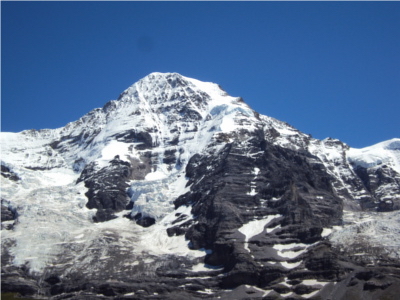
\includegraphics[width=0.45\linewidth]{./fig/hill1.jpg} &
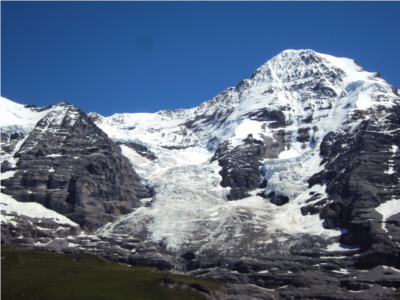
\includegraphics[width=0.45\linewidth]{./fig/hill2.jpg} \\
\end{tabular}
\caption{\label{fig:inputs} Input images to the image stitching algorithm.}
\end{figure}




Below is an outline of the steps you need to implement the algorithm.


\begin{enumerate}


\item \textbf{[0 points] Detect keypoints} The first step is to detect blobs in each image independently. You already implemented this in the first part. Remember to set the initial scale and threshold accordingly to get enough keypoints.
      
\item \textbf{[0 points] Feature extraction.} The next step is to extract feature descriptors on detected keypoints. The code to compute SIFT is included in the code base. The file \cmd{computeSift} takes an image and (x, y, radius) of $N$ blobs as input and return a matrix of size $N \times 128$ with 128 dimensional SIFT descriptor in each row.
%If you are using Matlab, the function uses different external libraries which are included in \cmd{mex} folder depending on the operating system. The first few lines in \cmd{evalStitching.m} sets up the environment variables in Matlab based on your operating system. The code has been tested to work on MATLAB 2019a version and earlier, and should work out of the box on Windows, MAC, and Linux platforms. Talk to the TA in case the mex files are not compatible with your operating system. If you are using Python, just install \cmd{opencv} using your favorite package manager.


\item \textbf{[10 points] Computing matches.} The next step is to compute matches between the two sets of features. Implement the function \cmd{matches = computeMatches(f1,f2)} that returns the best match of each feature \cmd{f1} to \cmd{f2} using the smallest sum-of-squared-differences. The input are two matrices \cmd{f1=dxN} and \cmd{f2=dxM} and the output is a array of size \cmd{Nx1} where each entry \cmd{matches(i)$\in$ [0,1,$\dots$,M]} is the closest feature in \cmd{f2} to the $i^{th}$ feature \cmd{f1(:,i)}, with \cmd{matches(i) = -1} indicating no matching.
%(using MATLAB's 1-starting indexing; for Python a no-match can be indicated by -1).


Considering only nearest neighbors returns many false matches. To refine the matches, compute the ratio of distance from the closest feature to the distance from the second closest feature and reject the matches with the ratio greater than a threshold. \href{http://www.cs.ubc.ca/~lowe/papers/ijcv04.pdf}{David Lowe's paper} suggest a threshold 0.8. Set \cmd{matches(i)=-1} if $i^{th}$ feature \cmd{f1(:,i)} fails on the ratio test.


You can visualize the matches using the \cmd{showMatches(im1, im2, c1, c2, matches)} function provided in the codebase. Figure~\ref{fig:match} shows the output of my implementation for reference.


\begin{figure}[h]
\centering
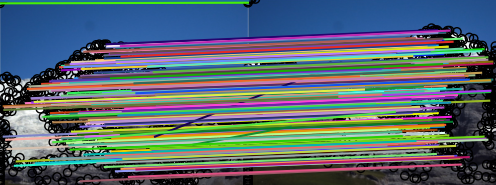
\includegraphics[width=0.75\linewidth]{./fig/matched.jpg}
% \vspace{-0.6in}
\caption{\label{fig:match} Matches between features.}
\end{figure}


\item \textbf{[25 points] Estimating affine transformation using \href{https://en.wikipedia.org/wiki/Random_sample_consensus}{RANSAC}.} The matching in the previous step is noisy and contains many outliers. Using RANSAC, estimate the affine translation that agrees with most matches (inliers). Implement the function \cmd{[inliers, transf] = ransac(matches, c1, c2)}. Here inliners is the indices of the inliner matches, transf is the estimated affine translation of $2\times 3$ matrix \cmd{$[m_1, m_2, t_1; m_3, m_4, t_2]$} between c1 and c2 (here they are blobs1 and blobs2 for image 1 and 2, repectively). You need at least three pairs of points to estimate the this. 

In Python, you might want to use \cmd{cv2.estimateAffine2D} in your implementation.

You can visualize the inlier matches using the \cmd{showMatches} function. Figure~\ref{fig:ransac_result} shows the output of my implementation for reference. The estimated affine transformation for this example is given as follows for your reference:


\begin{center}
$\begin{bmatrix}
0.9683 &  -0.0025 & -124.1000 \\
0.0103 & 0.9866 & 20.6513 \\
\end{bmatrix}$
\end{center}


\begin{figure}[h]
\centering
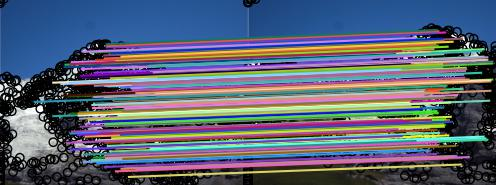
\includegraphics[width=0.75\linewidth]{./fig/ransac_result.jpg}
% \vspace{-0.6in}
\caption{\label{fig:ransac_result} Inliers obtained from RANSAC.}
\end{figure}


\begin{figure}[h]
\centering
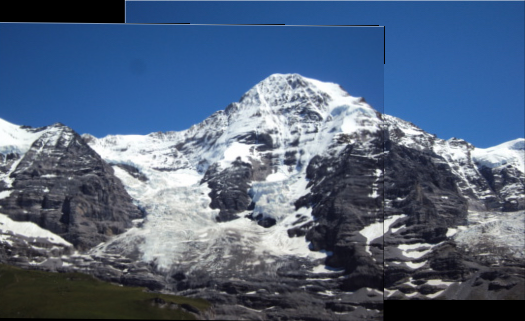
\includegraphics[width=0.8\linewidth]{./fig/stitch_result.jpg}
% \vspace{-0.6in}
\caption{\label{fig:output} Visualization of output.}
\end{figure}
\item \textbf{[0 points] Visualizing the stitched image.} Merge the images using \cmd{mergeImages(im1,im2, transf)} function provided in the codebase. The result is shown as Figure~\ref{fig:output}.
\end{enumerate}

\subsection{What to submit}
To get full credit for this part you have to
\begin{itemize}
\item Include your implementation of \cmd{computeMatches} and \cmd{ransac}.
\item Visualize the intermediate results and the output of each of the provided test image pairs. You can do this by setting the \cmd{exampleIndex} variable in the \cmd{evalStitching} file.
\item Report the estimated affine transformation for given test images.
\end{itemize}







 

\section{Report Writing and Presentation [10 points]}

Please use our homework latex as your template and organize your results reference to the homework latex.
Graders will penalize reports that are poorly written or fail to
present the results in a reasonable manner. You may find the
``verbatim" in Latex useful to include pasted code or from a file in
its raw format.
For example the code in a file
  \cmd{alignChannels.py} can be included in Latex by typing:
\begin{verbatim}
\verbatiminput{../code/alignChannels.py}.
\end{verbatim}


\end{document}
